% !TeX spellcheck = zh_CN
\documentclass[aps,pre,12pt,preprint,%
	onecolumn,showpacs,showkeys,nofootinbib]{revtex4-1}
%UnlimitedFonts
	\def\hmmax{0}
	\def\bmmax{0}
%SVG
	\usepackage{svg}
%Tables
	\usepackage{array,booktabs,tabularx,multirow}
	\newcolumntype{C}[1]{>{\hsize=#1\hsize%
		\centering\arraybackslash}X}
%Math&Fonts
	\let\latexointop\ointop
	\usepackage{mathtools,amssymb,bm % basics
		,physics,siunitx,slashed % physics
		,esint,nicefrac,extarrows,mathrsfs % more symbols
		,calligra,romannum,dsfont,fourier-orns % nice fonts
		,eqnarray,resizegather,empheq % more envs
		,relsize,stackengine % utils
	}
%	\usepackage{amsthm}
	\usepackage[scr=esstix]{mathalfa}
	\usepackage[only,sslash]{stmaryrd}
	%DisplaySetup
	\newcommand*\bbox[1]{\fbox{\hspace{1em}\addstackgap[5pt]{#1}\hspace{1em}}}
	\empheqset{box=\bbox}
	\mathtoolsset{showonlyrefs}
%Utils
	%Legacy \oint
	\let\ointop\undefined
	\let\ointop\latexointop
	%Calligra
	\DeclareMathAlphabet{\mathcalligra}{T1}{calligra}{m}{n}
	\DeclareFontShape{T1}{calligra}{m}{n}{<->s*[2.2]callig15}{}
	%CosmeticTweaks
	\newcommand\inlineeqno{\stepcounter{equation}\ (\theequation)}
	\newcommand\scalemath[2]{\scalebox{#1}{\mbox{\ensuremath{\displaystyle #2}}}}
	\newcommand\raisemath[2]{\raisebox{#1\depth}{${#2}$}}
	\newfontfamily\signature{Vladimir Script}
	\newcommand{\newparagraph}{\pagebreak[3]
		\noindent\hfil%
		\raisebox{-4pt}[10pt][10pt]{\leafright~\qquad~\leafleft}%
		\par\nopagebreak%
	}
%CustomCmds
	%Brackets
	\DeclarePairedDelimiter\ave{\langle}{\rangle}
	\DeclarePairedDelimiterX\inprod[2]{\langle}{\rangle}{#1,#2}
	%Basics
	\newcommand{\mbb}[1]{\mathbb{#1}}
	\newcommand{\mrm}[1]{\mathrm{#1}}
	\newcommand{\mcal}[1]{\mathcal{#1}}
	\newcommand{\mscr}[1]{\mathscr{#1}}
	\newcommand{\tup}[1]{\textup{#1}}
	\newcommand{\mop}[1]{\operatorname{#1}}
	%Extras
	\newcommand{\scriptr}{\mathcalligra{r}\,}
	\newcommand{\rvector}{\pmb{\mathcalligra{r}}\,}
	\newcommand{\hodgedual}{\operatorname{\star}}
	\newcommand{\dual}{\ \xlongleftrightarrow{\ \textrm{dual}\ }\ }
	\newcommand{\idty}{\mathds{1}}
	\newcommand{\proj}[1]{\operatorname{%
		proj_{\mathit{#1}}}}
	\newcommand{\propsim}{\mathbin{\ensurestackMath{
		\stackunder[2pt]{\propto}{\sim}
	}}}
	\newcommand{\textbox}[1]{\fbox{#1}}
	\newcommand{\pdd}[1]{\operatorname{\partial_{\mathnormal{#1}}}}
	\newcommand{\cdd}{\operatorname{D}\!}
	\newcommand{\cdv}[1]{\operatorname{%
		\nabla_{\!\mathit{#1}\!}}}
	\newcommand{\ldv}[1]{\operatorname{%
		\mcal{L}_{\!\mathit{#1}\!}}}
	\newcommand{\ric}[1]{\operatorname{%
		Ric}\!\pqty{#1}}
%Hacks
	% physics.sty <texmf-dist/tex/latex/physics/>
	% USER: more spacing around Dirac's middle vert
	\newcommand{\xmiddle}[1]{\mspace{1mu}\middle#1\mspace{1mu}}
	\DeclareDocumentCommand\innerproduct{ s m g }
	{ % Inner product
		\IfBooleanTF{#1}
		{ % No resize
			\IfNoValueTF{#3}
			{\vphantom{#2}\left\langle\smash{#2}\xmiddle\vert\smash{#2}\right\rangle}
			{\vphantom{#2#3}\left\langle\smash{#2}\xmiddle\vert\smash{#3}\right\rangle}
		}
		{ % Auto resize
			\IfNoValueTF{#3}
			{\left\langle{#2}\xmiddle\vert{#2}\right\rangle}
			{\left\langle{#2}\xmiddle\vert{#3}\right\rangle}
		}
	}

%Miscellaneous
%	\newcommand{\tabindent}{\hspace{2em}}
%FourierTransform
	\newcommand{\fourierf}{\mathscr F}
%Atoms
	\newcommand{\SrAtom}{\,\textsuperscript{90}\tup{Sr}\,}
	\newcommand{\Yatom}{\,\textsuperscript{90}\tup{Y}\,}
	\newcommand{\CsAtom}{\,\textsuperscript{137}\tup{Cs}\,}
	\newcommand{\CoAtom}{\,\textsuperscript{60}\tup{Co}\,}
	% Cool trick to include num: <tex.stackexchange.com/a/9719>
	\newcommand{\sFeCl}[1]{\tup{FeCl\textsubscript{#1}}}
	\newcommand{\sHIIO}{\tup{H\textsubscript{2}O}}
	\newcommand{\specWaterPlus}{\,\sHIIO\,(\sFeCl3)\,}
\begin{document}
%Basic Data
	\title{%
	\texstringonly{\hfil\\[2\baselineskip]}
	\sf\LARGE%
		核磁共振及其应用%
	\texstringonly{\vspace{3ex}}}
	\author{\fangsong\large%
		Bryan%
	\vspace{2mm}}
	\affiliation{\it%
		北京大学物理学院~~学号:\normalfont 1500066666\,}
	\date{\today}
	\keywords{核磁共振\ $g$因子\ 弛豫时间\ 尾波\ 瞬态现象}
	\email{masked_email_please_contact@github.com}

\begin{abstract}
\vspace{10mm}
\begin{spacing}{1.5}\normalsize
\setlength{\parskip}{.3\baselineskip}
%	200—300字,
%	说明用什么方法做了什么事,
%	由此得到什么结果和结论,
%	有何意义.
%	不用缩略词,不用第一人称.
%%%%%%%%%%%%%%%%%%%%%%%%%%%%%%%%
	实验首先得到了掺有 \sFeCl3 的 \sHIIO 样品中质子的核磁共振信号,由此验证了核磁共振现象;并在此基础上考察了不同实验条件对核磁共振信号的影响。
	
	在此基础上,实验中利用\specWaterPlus 样品质子共振信号和质子回旋频率的参考值对永久磁铁的磁场进行了校准;并进一步利用校准后的磁场测定了氟核的$g$因子。
	此外,通过估测信号的半宽度$\Delta\omega$, 估测了聚四氟乙烯中氟核的横向弛豫时间;最后观察并比较了纯水与\specWaterPlus 共振信号的差异。
\end{spacing}
\end{abstract}

\maketitle
\thispagestyle{titlepagestyle}

%	\item 课程实验报告应假定读者既不是已知全部实验细节的指导教师,也不是缺少专业知识的公众,而是同领域的实验研究者,或审稿人. 不能要求读者要在读过课程讲义后才能读懂课程实验报告.
%	\item 公式、图和表要分别用阿拉伯数字编列序号. 公式和图表要达到可发表的质量.
%	\item 凡不是自己独立思考得到的内容都应该引参考文献. 不能大段引用同一参考文献. 对复杂问题,应该优先考虑引用参考文献得到结果. 对简单一些的问题才鼓励独立思考.
%	\item 较长的推导和说明可以作为附件提交,不占用报告篇幅.
%	\item 思考题不是报告的组成部分. 应另起一页附在报告的最后.
\section{引言}
%%	研究论文引言一般包含以下内容:
%%	(1)所研究领域背景和现状;
%%	(2)有待研究的问题;
%%	(3)本研究的目的、主要内容和结果;
%%	(4)结果的意义.\par
%%	在写实验报告的引言时,同学可以假想自己是第一个做类似研究的人.\par
%%	引言一定要切合报告正文,不能漫无目的地介绍背景. 要快速地将读者引导到报告主题上,并作较深入的讨论.\par
%%	引言篇幅可以在较大范围内变化,但最长不应超过报告文字篇幅的1/3.\par
%%	引言撰写可以参考实验讲义,可以复述,但不能复制讲义上的任何一句话.\par
%%%%%%%%%%%%%%%%%%%%%%%%%%%%%%%
	磁矩非零的微观粒子处于外磁场中时会发生能级的Zeeman分裂,此时在垂直于磁场方向施加一个共振频率的交变磁场,可使粒子在相应的Zeeman能级之间发生共振跃迁,此即磁共振。

	1924年,W.\,Pauli提出了核磁矩和核自旋的概念,这为用电磁场和光谱研究原子核奠定了理论基础。测定核磁矩可以提供许多关于核结构与物质结构的信息;由于不同的原子核具有不同的磁矩,对应不同的共振信号,因此可以据此探测元素的种类。因此,如何精确地测量核磁矩成为一个重要的问题。
	
	1938年,I.\,I.\,Rabi首次在实验上观察到核磁共振现象\supercite{rabi1938new},并由此获得1944年诺贝尔物理学奖。
	Rabi的实验方法较为复杂,相应地,近代核磁共振技术于1946年被F.\,Bloch和E.\,M.\,Purcell的团队同时提出\supercite{PhysRev.69.37,PhysRev.70.474},现代核磁共振技术都是建立在其基础之上。他们二人也因此于1952年获得诺贝尔物理学奖。
	
	当今,核磁共振技术已在科学技术、医学、工程等领域得到广泛的应用。本实验采用与\cite{PhysRev.70.474}基本一致的实验设计,观察了核磁共振的现象,并在此基础上探究了实验条件的影响及核磁共振的基本应用(校准磁场、测定原子核的$g$因子)。
\section{理论}
	强外磁场$B_0$中,磁矩非零的原子核能级发生Zeeman分裂;当在垂直$B_0$方向加上强度适当的射频场(交变磁场),且频率为共振频率:
	\begin{equation}
		h\nu = \Delta E = \Delta\mu\,B_0
	\end{equation}
	时,原子核可被共振激发,并在此后跃迁回原能级并发出频率同为$\nu$的电磁波。可以通过探测电磁信号观察这一过程。
\clearpage

\setlength{\jot}{0pt}
	具体而言,引入核磁子$\mu_N = \pqty\big{\frac{e}{2m_p}}\,\hbar$, 有:
	\begin{equation}
		\mu = \gamma J
		= g_0\,\pqty\Big{\frac{q}{2m}}\,J
		= g\,\pqty\Big{\frac{e}{2m_p}}\,J
		= g\mu_N\,\frac{J}{\hbar}
	\end{equation}
	量子修正体现为上述$g$因子;进一步考虑角动量量子化$\Delta J = \hbar$, 则相应有$\Delta\mu = \gamma \Delta J = g\mu_N$, 从而有回旋频率:
	\begin{equation}
		\frac{\nu}{B_0}
		= \frac{g\mu_N}{2\pi\hbar}
		= \frac{\gamma}{2\pi}
	\label{eq:resonance_simplified}
	\end{equation}
	
	射频场频率与回旋频率对应时,原子核受激跃迁;注意射频场应当垂直于$B_0$方向,这可通过经典图像加以理解:磁矩在恒强$B_0$下发生Larmor进动,而扰动贡献的力矩为:
	\begin{equation}
		\bm{\tau} = \bm{\mu}\times\vb{B}'
	\end{equation}
	可见唯有$\vb{B}'\perp\vb{B_0}$, 方能使进动角$\theta$发生变化,进而使Zeeman能$E = -\bm{\mu}\cdot\vb{B}$发生改变,对应能级跃迁。
	
	\begin{figure}[!ht]
	\centering
	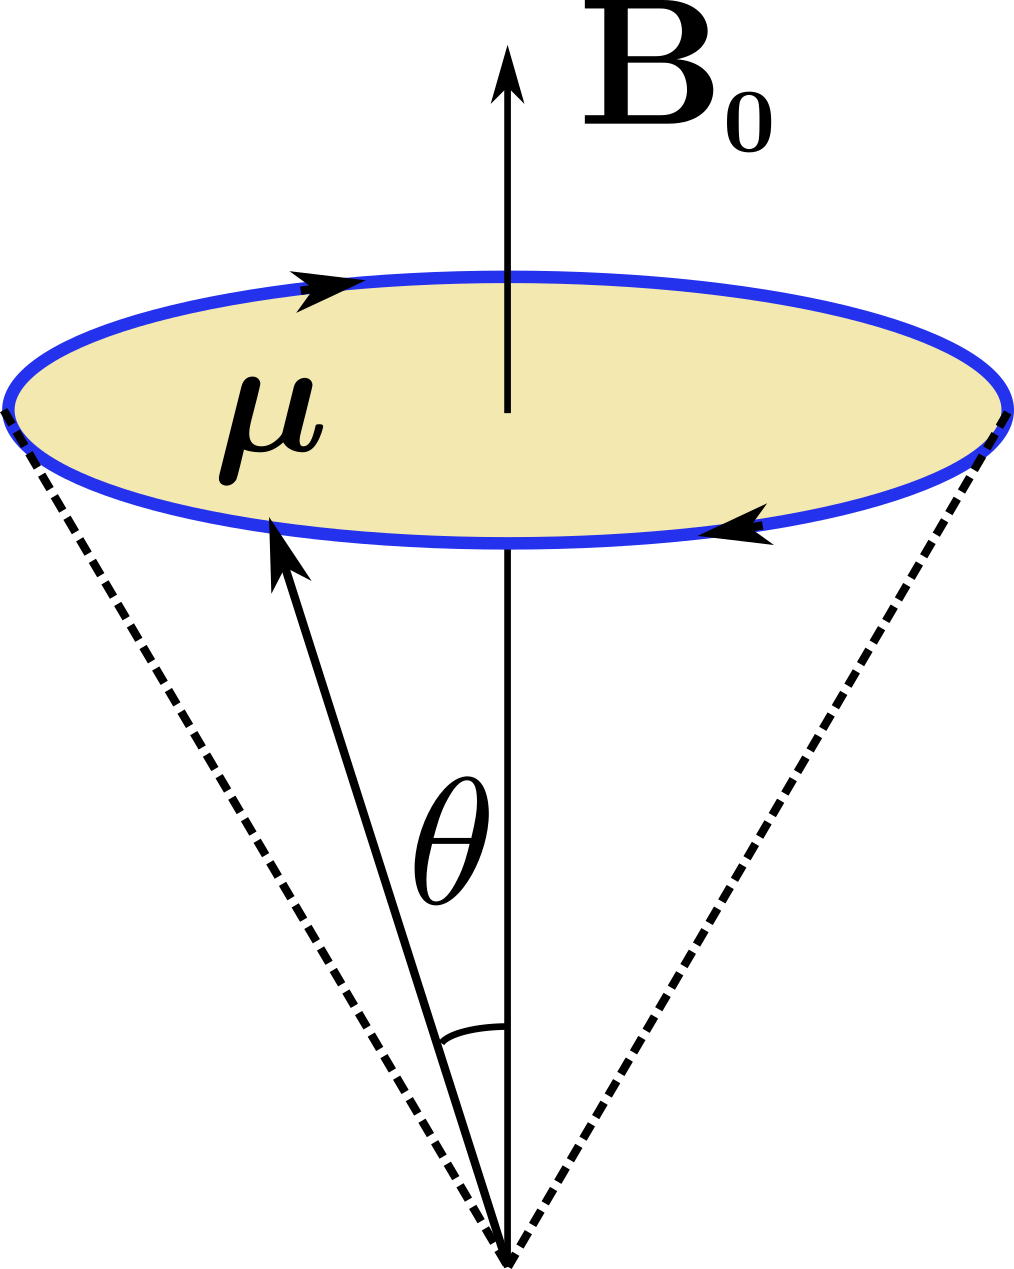
\includegraphics[width=.2\linewidth]{img/Larmor.png}
	\caption[Larmor进动图像]{%
		磁矩在外场下\tup{Larmor}进动的经典图像\footnote{%
			示意图据公共资源修改得到:
			\url{https://upload.wikimedia.org/wikipedia/commons/5/54/Larmor_01.svg}
		},参见\cite{textbook}. \\其中$\bm{\mu}$为粒子磁矩,$\vb{B_0}$为恒定外磁场。
	}\vspace{1ex}
	\end{figure}
\clearpage
	
	相反,若扰动$\vb{B}'\sslash\vb{B_0}$, 则只会改变进动速率,不改变进动角$\theta$, 这对应\cjkdot{能级结构}的变化;绝热近似(adiabatic approximation)下,并不会发生能级跃迁。
\restorejot
	
\newparagraph
	宏观上,样品磁化强度是众多微观磁矩之和:$\vb{M} = \sum_i \bm{\mu}_i$, 这也是实际测量的物理量;粒子数在上、下能级的分布大致为Boltzmann分布,能级间的粒子数差异$n_0$是观测到共振现象的关键。
	
	引入射频场后,当射频场作用与自旋--晶格驰豫达到动态平衡时,$n < n_0$. 特别当扰动场强$B'$很大时,共振吸收过强,此时能级间粒子数差异$n\to 0$, 出现饱和现象,难以观测到共振吸收。因此$B'$不能过大,应适当。
	
	此外,由于存在自旋--自旋相互作用,横向扰动$\vb{B}'$导致的非零$\vb{M}'(t)$将大致按指数规律衰减,衰减的时间尺度$T$即横向驰豫时间:
	\begin{equation}
		\dv{\vb{M}'}{t} = - \frac{\vb{M}'}{T}
	\end{equation}
	由含时微扰可知,$T$对应能级的寿命,其值可由吸收线宽$\Delta\omega$估测得到:$\frac{1}{2}\Delta\omega\,T\sim 1$. 事实上,实验中磁场的非均匀性会影响驰豫过程,故测得的$T$值实为等效驰豫时间。
	
	\newparagraph
	此外,实验中为观察到共振峰,必须使系统参数渐变地通过共振区间,这通过\textit{扫场、扫频}实现,参见后文。若这一过程充分地缓慢,则可近似地得到共振的稳态行为;不过实际上参数变化并不满足准静态要求,故实际上常常会观察到瞬态现象,其中最为典型的即为尾波。
	
	尾波是共振激发后$\vb{M}'$感生电动势频率与射频场频率间微小不同所造成的拍现象。显然,有效驰豫时间$T$越短,暂态现象越不明显;而磁场的不均匀性将使$T$值减小,故外磁场越均匀,尾波频次越多;可由此判断磁场均匀性。
\clearpage
\hfil\vspace{-1.2\baselineskip}
	\begin{figure}[!ht]
	\centering
	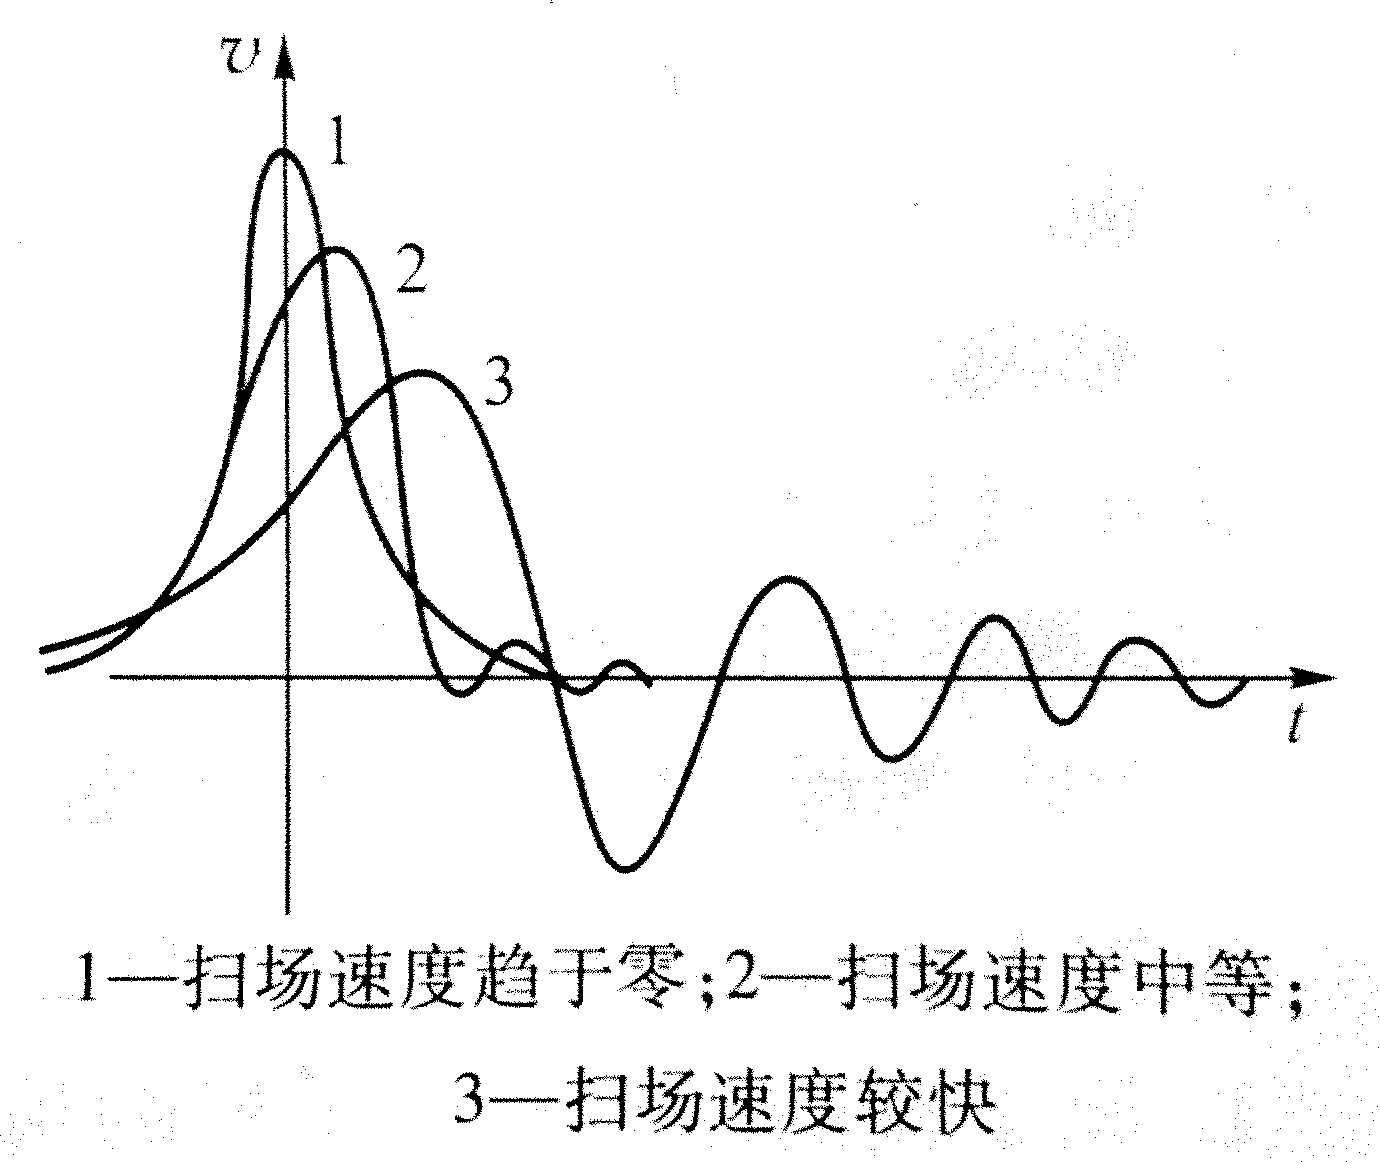
\includegraphics[width=.425\linewidth]{img/transient-b.jpg}
	\caption[尾波图像]{扫场速度不同时所观察到的核磁共振吸收信号,选自 \cite{textbook}. }
	\end{figure}
\FloatBarrier
\vspace{-1.2\baselineskip}
\section{实验装置}
\vspace{-1\baselineskip}
%%	在此部分需要将实验条件交待清楚到别人能重复你的实验结果的程度. 此外,还需表明你已尽了最大努力来提高实验精度和结果的可靠性. 简单的不确定度估计可以在此节给出,复杂一些的可以放到分析讨论部分.\par
%%	实验条件不仅是指直接影响实验结果的实验参量,而且还包括影响实验质量和可靠性的因素,如室温、空气湿度、基真空、原材料纯度等.\par
%%	作为教学实验报告,此节写详细一点没有坏处.\par
%%	成段有叙述,必要才分节。
%%%%%%%%%%%%%%%%%%%%%%%%%%%%%%%
	\begin{figure}[!ht]
	\centering
	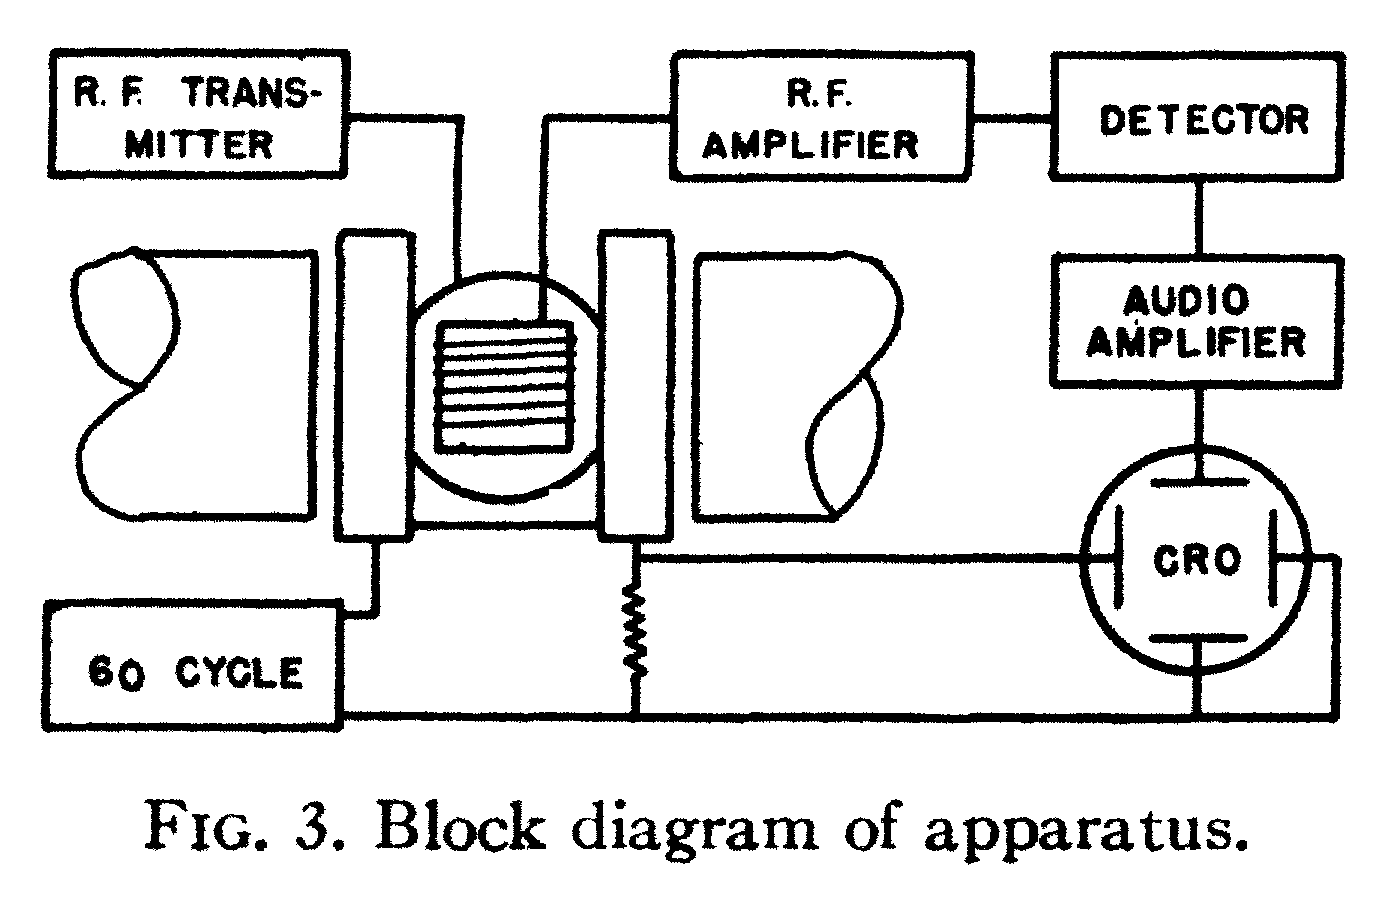
\includegraphics[width=.5\linewidth]{img/bloch_apparatus.png}
	\caption{核磁共振装置示意图,选自 \cite{PhysRev.70.474}. }
	\begin{explain}
		恒定磁场$B_0\approxeq\SI{0.5}{\tesla}$及扫场信号沿图示水平方向,恒磁场在均匀区范围内均匀性优于$10^{-5}$. 射频信号的产生与共振信号的接收均通过边限振荡器实现。
	\end{explain}
	\end{figure}
	
	实验采用NM-3型核磁共振装置,其工作原理与Bloch et al., 1946的实验设计 \cite{PhysRev.70.474} 基本一致,如图所示。
	
	射频磁场由振荡线圈(边限振荡器)产生,其产生的线偏振磁场可以分解为左旋、右旋圆偏振场,其中一个圆偏成分使样品共振激发;另一圆偏成分频率相反,远离共振区,其影响可以忽略。
\clearpage
	
	如前所述,实验中须使系统参数渐变地通过共振区间,以观察共振峰;若仅调整射频场频率而固定$B_0$不变,由于射频场频率旋钮的调节步长难以控制,远大于共振线宽,故极易错过共振区间。
	
	因此,实验中利用电磁铁在$B_0$上附加一个共线的 \SI{50}{\Hz} 交变磁场,相当于使恒磁场在$B_0 \pm\Delta B$之间连续变化,称为扫场。给定射频场频率,只要共振条件对应的场强在扫场变化范围内,就能观察到共振信号。
\section{结果与分析}
%	实验结果应尽量以图表的形式给出. 每一个图表都应该是完整的,即阅读图表时可以不必依赖正文.\par
%	依自己意愿,实验结果和对结果的分析讨论既可分为两节也可合在一节.\par
%
%	每个图一般包含:图名、轴名、轴、刻度、标尺、数据点、曲线、图例、标注和图注等部分. 应尽量让读者不看正文就能基本理解图的含意.\par
%	逐点测量得到的函数关系要同时用表格和图给出. 需要作比较的多条曲线要画在同一图上.\par
%	为避免读者在图表和正文间反复跳跃阅读,在正文中也要对图表作必要的说明.\par
%
%	对于预料之外的实验结果,必须首先小心证明其可靠性.读者只有在相信你的实验结果时才愿意花时间看你的分析.\par
%	必须用文字归纳整理出正式的实验结果或结论.可信的实验结果是课程报告最重要的内容.作为一个实验物理工作者,分析解释出错并不丢脸,实验结果不被采信则是致命的.\par
%	教学实验的结论往往是预先知道的. 所以,教师更关心的是你的说理过程. 一般说来,单由课内实验的结果不足以能得到明确的结论. 此时,你可以引用他人的研究结果来帮助帮助自己的论证,但必须注明出处. \par
%	确实不能得到明确结论时,可以给出几种可能结论并指出可以再做哪些实验来帮助作进一步的判断.\par
%	总之,分析讨论部分要做到: 论据要valid,论证要reasonable,结论要convincing.\par
%%%%%%%%%%%%%%%%%%%%%%%%%%%%%%
\subsection{观察\specWaterPlus 的共振信号}
	样品置于磁场中央,调整扫场电压$\sim\SI{100}{\V}$(与扫场强度正相关,故此后简记为扫场100),调整射频场频率直到示波器上可见共振峰,间隔$\sim\SI{10}{\ms}$(即每个 \SI{50}{\Hz} 的扫场周期有2个共振峰值)。在此基础上,
	\begin{enumerate}[label=(\arabic*),labelindent=0pt]
	\item 将射频场频率减小至共振频率以下,再逐渐增大,可见共振信号:
		\begin{itemize}
		\item \textbf{位置}:首先可见微弱的正弦背景,在其波谷附近出现共振峰,随后一份为二,直至等间距(\SI{10}{\ms})分布;随后又逐渐两两靠近,最终合二为一后消失。信号消失在正弦背景的波峰附近。
		\item \textbf{幅度}:出现信号后迅速增大,随后渐减至稳定(此时共振信号等间距);随后又渐增,在信号合二为一后骤减消失。
		\item \textbf{波形}:出现共振峰后,峰的右侧立即可见密集的尾波,一直如此直到共振信号消失;尾波的频率变化并不显著。
		\end{itemize}
	\vspace{2ex}\hspace{2em}\textbf{分析}:这正是射频场频率通过$B_0\pm\Delta B$共振区间的过程,其中微弱的正弦背景正是扫场信号。具体而言:\clearpage
		\begin{itemize}
		\item 随射频场频率增大,$B_0-\Delta B$首先满足共振条件,随后在每个扫场周期中,有2个磁场值满足共振条件,故有共振峰一分为二;在$B_0+\Delta B$时最后满足共振条件,共振信号在此合二为一后消失。
		\item 两共振峰接近时互相增强,因此幅度大。特别地,当共振峰等 \SI{10}{\ms} 间距时,对应的共振磁场大致是$B_0$. 此外,尾波密集表明磁场充分均匀。
		\end{itemize}
	\vspace{.5ex}
	\item 将扫场调至250, 调射频场频率使共振信号等 \SI{10}{\ms} 间距,减小扫场,可见信号:
		\begin{itemize}
		\item \textbf{位置}:两两靠近,最终合二为一消失。
		\item \textbf{幅度}:渐增,在信号合二为一后骤减消失。
		\item \textbf{波形}:初始正弦背景显著,随后减弱;始终可见明显的尾波,不过扫场越弱,尾波越稀疏。
		\end{itemize}
	\vspace{.5ex}\hspace{0em}\textbf{分析}:
		\begin{itemize}
		\item 相对扫场幅度$\Delta B$而言,初始的共振位置大致处在$B_0\pm\Delta B$区间的中心;不过,随$\Delta B$减小,共振磁场$B$与$B_0$的间距$\abs{B-B_0}$不变,但由于区间长度$2\Delta B$减小,共振点开始\cjkdot{相对偏离}区间中点;直到$\Delta B<\abs{B-B_0}$时,$B$完全落在了共振区间之外,此时信号消失。若随之调整共振频率使信号始终间隔 \SI{10}{\ms}, 则可使$B$越加精确地靠近$B_0$, 由此可实现精确测量。
		\item 如上所述,尾波实为共振频率与射频场频率有微小差异时的拍现象;$\Delta B$减小即缩小了共振频范围$\Delta\omega$, 频率越接近,拍频越小,即尾波越疏。
		\end{itemize}
	\vspace{.5ex}
	\item 将扫场调至50, 调射频场频率使共振信号等 \SI{10}{\ms} 间距,从最左端到最右端移动样品,可见信号:
		\begin{itemize}
		\item \textbf{位置}:不变。
		\item \textbf{幅度}:先增大后减小,最大在 \SI{1.8}{\cm} 刻度附近。
		\item \textbf{波形}:最先没有尾波,随后出现疏且少的尾波,逐渐变密变多,最多在 \SI{1.8}{\cm} 刻度附近;此后又渐疏渐少至消失。
		\end{itemize}\clearpage
	\vspace{0ex}\hspace{2em}\textbf{分析}:左右移动样品相当于改变$B_0$的强度和均与性;在两侧$B_0$弱且不均匀,故共振峰幅度小。此外,如前所述,$B_0$的不均匀性将减小等效驰豫时间$T$, 这不利于尾波的形成,故样品在两侧时不可见尾波。由此可知,\SI{1.8}{\cm} 刻度附近的磁场最为均匀。%
	\vspace{-2ex}
	\item 样品重新置于 \SI{1.8}{\cm} 刻度处,保持射频场频率不变,由小到大调整其幅度,可见信号:
		\begin{itemize}
		\item \textbf{位置}:不变;事实上,实验中调整射频场幅度后其频率会发生漂移,正是通过调整令信号等 \SI{10}{\ms} 间距不变以控制频率不变。
		\item \textbf{幅度}:先增大后减小,最大在射频场幅度 \numrange{6}{7} 附近。
		\item \textbf{波形}:无明显变化。
		\end{itemize}
	\vspace{0ex}\hspace{2em}\textbf{分析}:射频场较小时,幅度越大共振跃迁越显著,对应信号幅度增大;射频场过大时,发生前述饱和现象,信号幅度反之减小。
	\end{enumerate}
\subsection{利用核磁共振校准磁场}
	在前述实验所确定的最优参数下,利用前述减小扫场幅度的手段控制精度,以校准$B_0$. 具体而言,给定质子的$\frac{\gamma}{2\pi}$值\footnote{%
		参考值出自 \cite{textbook}. 
	},利用共振条件 \eqref{eq:resonance_simplified} 及$\Delta B$确定$B_0$及其不确定度。实测共振峰等 \SI{10}{\ms} 间距时,有$B_0$对应:
	\begin{equation}
		\nu \simeq \SI{21.099321}{\MHz}
	\end{equation}
	相应有共振区间对应的频率上下限
		$\nu_{\max} \simeq \SI{21.109435}{\MHz},\,
		\nu_{\min} \simeq \SI{21.092129}{\MHz}$, 
	这给出磁场的不确定度估计:
	\begin{equation}
		\sigma \sim \frac{\Delta B}{10}
			\simeq \frac{1}{10} \frac{\nu_{\max} - \nu_{\min}}{2}
			\bigg/ \frac{\gamma}{2\pi}
			\sim \num{2e-5}
	\end{equation}
\clearpage
	综上,可得:
	\begin{equation}
		B_0 = \SI{.49556(2)}{\tesla}
	\end{equation}
	相对不确定度$\sim\num{4e-5}$. 
\subsection{测定聚四氟乙烯中氟核的$g$因子}
	完全类似上述实验,利用已校准的$B_0$, 可测定未知原子核的$g$因子。考察聚四氟乙烯中的氟核,已知$\frac{\nu_N}{\hbar}$, 由 \eqref{eq:resonance_simplified} 有$g = \frac{\nu}{B_0}\big/\frac{\mu_N}{\hbar}$, 而$B_0$对应:
	\begin{equation}
		\nu \simeq \SI{19.854315}{\MHz}
	\end{equation}
	相应有共振区间对应的频率上下限
		$\nu_{\max} \simeq \SI{19.879176}{\MHz},\,
		\nu_{\min} \simeq \SI{19.830215}{\MHz}$, 
	误差传递按相对误差的方和根加以估算,可得相对不确定度$\sim\num{1e-4}$, 
	\begin{equation}
		g = \num{5.2560(5)}
	\end{equation}
\subsection{测定聚四氟乙烯中氟核的横向驰豫时间$T$}
	由扫场为$X$, 可作出共振峰随磁场的关系,得相对扫场范围的半宽:
	\begin{equation}
		\kappa \simeq \num{0.04142857}
	\end{equation}
	而共振磁场与射频场线性相关,即实际有$\kappa = \frac{\Delta\nu}{\nu_{\max} - \nu_{\min}}$, 这里$\nu_{\max}, \nu_{\min}$按前述步骤测得;又$\frac{1}{2}\Delta\omega\,T\sim 1$, 可得:
	\begin{equation}
		T \sim \frac{1}{\pi\kappa(\nu_{\max} - \nu_{\min})}
		\sim \SI{39.0}{\us}
	\end{equation}
\subsection{观察纯水样品的核磁共振现象}
	前述实验中的水样品掺有\sFeCl3, 作为比较,实验中最后观测了纯水样品的核磁共振现象;相对\specWaterPlus 而言,纯水样品的共振信号极弱,在对\specWaterPlus 而言的最佳实验条件下,纯水样品难以看到共振峰,唯有当射频场幅度调高至9时方可见信号;且此时信号幅度也仅为背景噪声的两倍左右,无法明显地看出是否有尾波。
	
	\textbf{分析}:\specWaterPlus 样品由于掺入顺磁剂$\tup{Fe}^{3+}$离子,使样品中局域磁场增强,显著减小了样品的驰豫时间,从而使得共振峰得以增强。
\section{结论}
%%%	首先要给出实验结果,然后再给出由实验结果分析得到的结果和结论。此部分给出的内容要比摘要中的全面,用词要更准确。\par
%%%%%%%%%%%%%%%%%%%%%%%%%%%%%%%
	本实验重现了多种样品的核磁共振现象,观察并分析了实验参数对核磁共振现象的影响,得到了核磁共振测定的最佳条件:尽可能小的扫场幅度、均匀且恒强的静磁场及适当的射频场频率。在此基础上,相对精确地标定了磁场、测定了聚四氟乙烯中氟核的$g$因子及横向驰豫时间,了解了利用核磁共振现象进行精密测量的基础知识。
\section{致谢}
%	此部分感谢同组人...和对实验和报告有帮助的人。
%%%%%%%%%%%%%%%%%%%%%%%%%%%%%%
	感谢黄斐增老师的细致指导和耐心帮助;感谢 \TeX\, - \LaTeX\, Stack Exchange\footnote{%
		\url{https://tex.stackexchange.com/}
	}, 助我解决了众多排版问题。
\clearpage

\setlength{\bibsep}{2pt}
\linespread{1.2}\selectfont
\bibliographystyle{../BibStyle/gbt-7714-2015-numerical}
\bibliography{../BibStyle/Textbook,bib/Ref}

\clearpage
\end{document}